\documentclass[11pt]{article}

% Language setting
\usepackage[turkish]{babel}
\usepackage{pythonhighlight}

\usepackage[a4paper,top=2cm,bottom=2cm,left=2cm,right=2cm,marginparwidth=2cm]{geometry}

% Useful packages
\usepackage{amsmath}
\usepackage{graphicx}
\usepackage[colorlinks=true, allcolors=blue]{hyperref}
\usepackage{verbatim}
\usepackage{fancyhdr} % for header and footer
\usepackage{titlesec}
\usepackage{parskip}

\setlength{\parindent}{0pt}

\titleformat{\subsection}[runin]{\bfseries}{\thesubsection}{1em}{}

\pagestyle{fancy} % activate the custom header/footer

% define the header/footer contents
\lhead{\small{23BLM-4014 Yapay Sinir Ağları Ara Sınav Soru ve Cevap Kağıdı}}
\rhead{\small{Dr. Ulya Bayram}}
\lfoot{}
\rfoot{}

% remove header/footer on first page
\fancypagestyle{firstpage}{
  \lhead{}
  \rhead{}
  \lfoot{}
  \rfoot{\thepage}
}
 

\title{Çanakkale Onsekiz Mart Üniversitesi, Mühendislik Fakültesi, Bilgisayar Mühendisliği Akademik Dönem 2022-2023\\
Ders: BLM-4014 Yapay Sinir Ağları/Bahar Dönemi\\ 
ARA SINAV SORU VE CEVAP KAĞIDI\\
Dersi Veren Öğretim Elemanı: Dr. Öğretim Üyesi Ulya Bayram}
\author{%
\begin{minipage}{\textwidth}
\raggedright
Öğrenci Adı Soyadı: Hatice Hesna ÇALIŞKAN\\ % Adınızı soyadınızı ve öğrenci numaranızı noktaların yerine yazın
Öğrenci No: 190401007
\end{minipage}%
}

\date{14 Nisan 2023}

\begin{document}
\maketitle

\url{https://github.com/hesnacaliskan/Artifical_Neural_Networks_Midterm_Exam_LatEx}

\section{(Toplam 10 Puan) Hopfield Networks:}

\subsection{(2 Puan)} \textbf{ChatGPT’ye size Hopfield Network’ler ile ilgili detaylı bilgi vermesini isteyin. Sorduğunuz soruyu, ChatGPT'nin çıkartığı cevabı aşağı koyun. Bu cevapta anlamadığınız terimleri de ChatGPT’ye sorup, sorduğunuz soruları ve ChatGPT’nin verdiği cevapları da sırayla aşağı koyun.}
 
\begin{itemize}
    \item \textbf{Hopfield Network’ler ile ilgili detaylı bilgi verir misin?}
\end{itemize}

Elbette, Hopfield ağları, yapay sinir ağları sınıfında yer alan bir tür geri beslemeli ağdır. Bu ağlar, asenkron ve geri beslemeli bir yapıya sahiptir ve öğrenme ve hatırlama işlevleri için kullanılırlar.

Hopfield ağları, temel olarak nöronlar arasındaki bağlantıların bir matrisle ifade edildiği bir modeldir. Bu matris, ağırlık matrisi olarak bilinir ve nöronların birbirleriyle nasıl bağlandığını gösterir. Ağırlık matrisi, nöronların etkileşimleri arasındaki güçleri gösteren simetrik bir matristir.

Ağın çalışma prensibi, bir girdi verildiğinde, ağın kendisi tarafından belirlenen bir iterasyon işlemi ile çıkışı hesaplamasıdır. Bu iterasyonlar, ağırlık matrisinin özelliklerine göre gerçekleşir. Her iterasyonda, her nöron, diğer nöronların çıkışlarına göre bir çıkış değeri hesaplar ve bu değerler, ağın sonraki adımda hangi nöronların aktive olacağına karar verir.

Hopfield ağları, öğrenme ve hatırlama işlevleri için kullanılabilir. Öğrenme, ağırlık matrisinin bir veri kümesi üzerinde eğitilmesini içerir. Bu eğitim, ağırlık matrisinin simetrik olmasını ve belirli bir enerji fonksiyonuna sahip olmasını sağlar. Hatırlama işlevi, ağırlık matrisine kaydedilen örüntüleri hatırlama kapasitesine sahip olmayı içerir. Bu örüntüler daha sonra girdi olarak verilebilir ve ağ, örüntünün en yakın hafızadaki örneğine yakın bir çıkış üretir.

Hopfield ağları, özellikle düşük boyutlu verilerde başarılı olabilir. Örneğin, rakam tanıma veya yüz tanıma gibi görsel tanıma görevleri için kullanılabilirler. Ancak, büyük boyutlu veriler için Hopfield ağları yetersiz kalabilir ve daha büyük yapay sinir ağları, örneğin evrişimsel sinir ağları kullanılması gerekebilir.

\begin{itemize}
    \item \textbf{ Evrişimsel sinir ağları nedir ?}
\end{itemize}

Evrişimsel sinir ağları (CNN), görsel verileri işlemek için kullanılan bir tür yapay sinir ağıdır. Bu ağlar, nöronların birbirleriyle bağlantıları arasındaki ağırlıkların otomatik olarak öğrenildiği bir öğrenme süreci ile eğitilir.

CNN'ler, görsel verilerin özelliklerini algılamak için tasarlanmıştır. Bu ağlar, özellikle görüntü tanıma, nesne tespiti, yüz tanıma ve doğal dil işleme gibi alanlarda başarılıdır.

CNN'lerin temel özelliklerinden biri, evrişim işlemidir. Bu işlem, bir filtre ya da çekirdek olarak adlandırılan küçük bir matrisin görüntü üzerinde hareket ettirilerek görüntünün farklı bölgelerindeki özelliklerin tespit edilmesini sağlar. Bu filtreler, özellik çıkarımı için kullanılır ve daha sonra daha büyük özelliklere veya nesnelere dönüştürmek için bir ara katman olarak kullanılır.

CNN'ler ayrıca, ağın derinleştirilmesi yoluyla da daha karmaşık özellikleri öğrenmek için kullanılabilir. Bu derinleştirme, ağın daha fazla katman ekleyerek, her katmanda farklı özellikleri öğrenerek yapılır.

Sonuç olarak, evrişimsel sinir ağları, görsel verilerin özelliklerini algılamak ve nesne tespiti, yüz tanıma ve doğal dil işleme gibi görevlerde başarılı olmak için tasarlanmıştır. Bu ağlar, filtreleme işlemi ve derinleştirme özellikleri sayesinde, doğru sonuçlar elde etmek için çok sayıda veri üzerinde eğitilebilirler.

\begin{itemize}
    \item \textbf{Hopfield Ağlarını neden bilmemiz gerekmektedir ?}
\end{itemize}

Hopfield ağları, yapay sinir ağı alanında oldukça önemli bir konudur ve bu nedenle bilmemiz gerekmektedir. İşte Hopfield ağlarını öğrenmek için bazı nedenler:

Bellek Yönetimi: Hopfield ağları, bellek yönetimi için kullanılabilir. Bu ağlar, depolanmış örüntüleri hatırlama ve tanıma yeteneğine sahiptirler. Bu özellikleri sayesinde, Hopfield ağları, bilgisayarlar ve diğer yapay zeka uygulamaları için önemli bir bellek yönetimi aracıdır.

Veri Sıkıştırma: Hopfield ağları, veri sıkıştırma için kullanılabilir. Bu ağlar, yüksek boyutlu verileri daha düşük boyutlu örüntüler halinde sıkıştırmak için kullanılabilirler. Bu özellikleri, veri saklama ve iletişim açısından büyük bir avantaj sağlar.

Öğrenme Teorisi: Hopfield ağları, öğrenme teorisi ve sinir ağıların temel prensipleri hakkında önemli bir anlayış sağlar. Bu ağlar, nöronların nasıl çalıştığı ve birbirleriyle nasıl etkileşimde bulunduğu hakkında fikir verir.

İşlemcilik: Hopfield ağları, paralel işlemcilerde işlem yapmak için de kullanılabilirler. Bu özellikleri, büyük veri işleme ve yapay zeka uygulamaları gibi yoğun hesaplama gerektiren işlemlerde büyük bir avantaj sağlar.

Sonuç olarak, Hopfield ağları, bellek yönetimi, veri sıkıştırma, öğrenme teorisi ve paralel işlemcilik gibi çeşitli uygulamalar için kullanılabilecek önemli bir araçtır. Bu nedenle, Hopfield ağlarını bilmek, yapay zeka ve bilgi işlem alanlarında çalışanlar için faydalı bir bilgidir.

\begin{itemize}
    \item \textbf{Hopfield Ağları gerçek hayatta kullanılır mı ?   }
\end{itemize}

Evet, Hopfield ağları gerçek hayatta birçok alanda kullanılmaktadır. İşte Hopfield ağlarının gerçek hayatta kullanımına örnekler:

Optik karakter tanıma (OCR): Hopfield ağları, optik karakter tanıma (OCR) sistemlerinde kullanılır. Bu sistemler, belgelerdeki yazıları dijital formatta tanımlamak ve okumak için kullanılır. Hopfield ağları, belirli bir yazı tipinin özelliklerini öğrenerek, farklı yazı tiplerindeki karakterleri tanımlayabilir.

Nesne tanıma: Hopfield ağları, nesne tanıma sistemlerinde de kullanılır. Bu sistemler, görüntülerdeki nesneleri tanımlamak ve sınıflandırmak için kullanılır. Hopfield ağları, nesnelerin özelliklerini öğrenerek, doğru sınıflandırmalar yapabilir.

Yapay zeka: Hopfield ağları, yapay zeka sistemlerinde kullanılır. Özellikle, bellek yönetimi, veri sıkıştırma ve paralel işlemcilik gibi alanlarda kullanılır. Bu ağlar, yapay sinir ağları arasında en popüler olanlarından biridir ve yapay zeka uygulamalarında önemli bir rol oynarlar.

Biyolojik uygulamalar: Hopfield ağları, biyolojik uygulamalarda da kullanılır. Özellikle, sinir ağları ve nöronların çalışması hakkında daha iyi bir anlayış elde etmek için kullanılırlar.

Ekonomi ve finans: Hopfield ağları, ekonomi ve finans alanlarında da kullanılır. Özellikle, hisse senedi fiyatları ve piyasa trendleri gibi finansal verilerin analizinde kullanılırlar.

Bu nedenlerle, Hopfield ağları gerçek hayatta birçok alanda kullanılır ve önemli bir rol oynarlar.


\subsection{(8 Puan)} \textbf{ChatGPT’nin açıklamalarından ne anladığınızı buraya kendi kelimelerinizle özetleyin. Örneğin ``Hopfield Network nedir? Ne işe yarar? Neden bilmemiz gerekir bunu? Gerçek hayatta kullanılıyor mu?'' gibi. Anlamadığınız kısımlar varsa ve ChatGPT’nin açıklamaları yeterli gelmezse internet dahil farklı kaynaklardan araştırıp, bilgilerin doğruluğunu sorgulamakta serbestsiniz. Konuyu doğru anlayıp anlamamanız puana etki edecektir. Kullandığınız kaynakları da belirtin!}

Hopfield ağlarının özelliklerini ve kullanım alanlarını bilmek, yapay sinir ağı konusunda genel bir anlayışa sahip olmamızı sağlar. Bu ağlar, geri beslemeli bir yapıya sahip olduğu için, nöronların etkileşimlerini modelleme konusunda önemlidir. Ayrıca, öğrenme ve hatırlama işlevleri için kullanıldığından, bellek ve veri işleme alanlarında da tercih edilmektedir..

Hopfield ağları,özellikle, düşük boyutlu verilerin işlenmesi ve tanınması için etkilidirler. Bununla birlikte, büyük boyutlu veriler için Evrişimsel Sinir Ağları gibi daha büyük yapay sinir ağları kullanılması gerekebilir.

Hopfield ağları, ayrıca, bağlantılı sistemlerin (neural networks), özellikle geri beslemeli sistemlerin incelenmesi için de önemlidir. Bu ağlar, nöronlar arasındaki etkileşimleri modellediği için, daha karmaşık bağlantılı sistemlerin çalışması hakkında bilgi sağlar. 

Hopfield ağları, gerçek hayatta otik karakter tanıma, nesne tanıma, biyoloji ve finans gibi alanlarda kullanılmaktadır.

\section{(Toplam 10 Puan) Boltzman Machine:}

\subsection{(2 Puan)} \textbf{ChatGPT’ye size Boltzman Machine ilgili detaylı bilgi vermesini isteyin. Sorduğunuz soruyu, ChatGPT'nin çıkartığı cevabı aşağı koyun. Bu cevapta anlamadığınız terimleri de ChatGPT’ye sorup, sorduğunuz soruları ve ChatGPT’nin verdiği cevapları da sırayla aşağı koyun.}

\begin{itemize}
    \item \textbf{Boltzman Machine ilgili detaylı bilgi verir misin?}
\end{itemize}
Bir Boltzmann makinesi (Boltzmann machine), sinir ağı ve makine öğrenimi alanında yaygın olarak kullanılan bir tür yapay sinir ağıdır. Boltzmann makineleri, bağlantıların olasılıkla ağırlıklı olduğu ve her bir düğümün durumunun 1 veya 0 olabileceği bir modeldir. Bu tür bir model, birbirleriyle bağlantılı olan birçok sinir hücresinin aktivasyonlarını modeller.

Boltzmann makineleri, birçok farklı uygulamada kullanılır, özellikle de veri önişlemesi, model seçimi ve doğrulama, özellikle de hedefsiz öğrenme, gruplama, kalıplaşma, düzenleme, ve azaltma işlemlerinde. Bu makine öğrenimi teknikleri, özellikle de yüksek boyutlu verilerde kullanılmak üzere tasarlanmıştır.

Bir Boltzmann makinesi, birçok gizli ve görülebilir düğüm (nöron) içerir. Gizli düğümler birbirleriyle bağlantılıdır ve bağlantıları belirleyen ağırlıklar, makinenin öğrenmesi gereken değişkenlerdir. Görülebilir düğümler, makinenin giriş verilerini alır ve diğer düğümlerle bağlantılıdır.

Bir Boltzmann makinesinin çalışması, enerji fonksiyonları ve Gibbs dağılımları gibi istatistiksel mekanik kavramlarından yararlanır. Bir Boltzmann makinesinde, bir veri noktasının olasılığı, makinedeki her bir düğümün durumunun olasılığına bağlıdır. Enerji fonksiyonu, her bir düğümün durumunu ve her bir bağlantının ağırlığını içerir. Makine, ağırlıkların doğru bir şekilde ayarlanmasıyla öğrenir ve daha sonra verileri sınıflandırmak veya özelliklerini çıkarmak için kullanılabilir.

Bir Boltzmann makinesi, yüksek boyutlu verilerde özellikle başarılı olabilir. Ancak, daha büyük veri kümelerinde çalışırken, eğitim süresi artabilir ve bazı durumlarda öğrenme verimliliği azalabilir. Bununla birlikte, Boltzmann makineleri, birçok farklı alanda kullanılmakta ve veri analizi ve örüntü tanıma için güçlü bir araç olmaktadır.

\begin{itemize}
    \item \textbf{Boltzman Makinelerinin hangi durumda öğrenme verimliliği azalabilir?}
\end{itemize}

Boltzmann makineleri, büyük boyutlu verilerde özellikle başarılı olabilir, ancak öğrenme verimliliği bazı durumlarda azalabilir. Öğrenme verimliliği, aşağıdaki durumlarda azalabilir:

Veri setinin büyüklüğü: Boltzmann makineleri, büyük veri kümeleriyle çalışırken, eğitim süresi artabilir ve öğrenme verimliliği azalabilir.

Aşırı öğrenme (overfitting): Boltzmann makineleri, modelin aşırı öğrenmesine eğilimli olabilir. Bu, modelin eğitim verilerinde iyi performans göstermesine rağmen, yeni verilerde kötü performans göstermesine neden olabilir.

Ağın karmaşıklığı: Boltzmann makinelerinin ağırlıklarının doğru bir şekilde ayarlanması, özellikle büyük ve karmaşık ağlar için zor olabilir. Bu nedenle, ağın karmaşıklığı arttıkça, öğrenme verimliliği azalabilir.

Ağın özellikleri: Boltzmann makineleri, bazı tür veriler için daha iyi performans gösterirken, diğer tür veriler için daha az etkili olabilir. Örneğin, imge verileri için daha iyi performans gösteren bir Boltzmann makinesi, doğal dil işleme verileri için daha az etkili olabilir.

İlk parametre seçimi: Boltzmann makinesinin eğitim verilerine göre ilk parametreleri belirlemek önemlidir. Yanlış parametre seçimi, öğrenme verimliliğini azaltabilir.

Bu nedenlerden dolayı, Boltzmann makineleri kullanmadan önce, verilerin doğası ve boyutu dikkate alınarak modelin uygunluğu ve öğrenme verimliliği değerlendirilmelidir.

\begin{itemize}
    \item \textbf{Boltzman Makinelerini ne işe yarar?}
\end{itemize}

Boltzmann makineleri, makine öğrenmesinde ve yapay zeka araştırmalarında kullanılan bir tür olasılıksal grafik modelidir. Bu makineler, bir veri setindeki örüntüleri ve ilişkileri otomatik olarak öğrenir ve bu öğrenme sonucunda yeni verileri sınıflandırabilir, özellikle ağır öğrenme (deep learning) alanında kullanılır.

Boltzmann makineleri, genellikle veri sıkıştırma, boyut azaltma, veri segmentasyonu, veri kümeleme, özellik seçimi ve model seçimi gibi makine öğrenmesi problemlerinin çözülmesinde kullanılır. Özellikle, derin öğrenme alanında Boltzmann makineleri, sinir ağları için önemli bir bileşen olarak kullanılmaktadır.

Boltzmann makineleri ayrıca, doğal dil işleme, görüntü işleme, tıbbi teşhis, finansal analiz, robotik, oyun teorisi, kimya ve fizik gibi birçok uygulama alanında da kullanılır.

Bununla birlikte, Boltzmann makineleri, büyük ve karmaşık veri setleri üzerinde çalışırken bazı zorluklarla karşılaşabilir ve eğitim süresi uzun olabilir. Bu nedenle, verilerin doğası ve boyutu dikkate alınarak modelin uygunluğu ve öğrenme verimliliği değerlendirilmelidir.

\begin{itemize}
    \item \textbf{Boltzman Makineleri gerçek hayatta kullanılıyor mu?}
\end{itemize}

Evet, Boltzmann makineleri gerçek hayatta birçok alanda kullanılmaktadır. Özellikle, makine öğrenmesi ve yapay zeka alanlarında yaygın olarak kullanılmaktadır. Aşağıda bazı örnekleri verilmiştir:

Doğal Dil İşleme (NLP): Boltzmann makineleri, metin verilerinin işlenmesinde kullanılır. Örneğin, kelime dağılımı modelleri, dil modellemesi ve metin sınıflandırma için kullanılır.

Görüntü İşleme: Boltzmann makineleri, görüntülerin öznitelik çıkarımında ve tanıma gibi görevlerde kullanılır.

Robotik: Boltzmann makineleri, robotik sistemlerin öğrenmesinde kullanılır. Örneğin, robotların nesneleri tanıması veya görevlerini yerine getirmesi için kullanılabilir.

Finans: Boltzmann makineleri, finansal verilerin analizi ve risk yönetimi gibi alanlarda kullanılır.

Tıp: Boltzmann makineleri, tıbbi görüntüleme, teşhis ve tedavi planlaması gibi alanlarda kullanılır.

Kimya: Boltzmann makineleri, kimyasal reaksiyonların modellenmesinde ve moleküler yapıların tasarımında kullanılır.

Fizik: Boltzmann makineleri, karmaşık fiziksel sistemlerin modellenmesinde ve simülasyonunda kullanılır.

Bu örneklerin yanı sıra, Boltzmann makineleri diğer birçok alanda da kullanılmaktadır ve makine öğrenmesi ve yapay zeka alanındaki araştırmaların önemli bir bileşenidir.


\subsection{(8 Puan)} \textbf{ChatGPT’nin açıklamalarından ne anladığınızı buraya kendi kelimelerinizle özetleyin. Örneğin ``Boltzman Machine nedir? Ne işe yarar? Neden bilmemiz gerekir bunu? Gerçek hayatta kullanılıyor mu?'' gibi. Anlamadığınız kısımlar varsa ve ChatGPT’nin açıklamaları yeterli gelmezse internet dahil farklı kaynaklardan araştırıp, bilgilerin doğruluğunu sorgulamakta serbestsiniz. Konuyu doğru anlayıp anlamamanız puana etki edecektir. Kullandığınız kaynakları da belirtin!}

Boltzmann makineleri, olasılıksal bir grafik modelidir ve makine öğrenmesi alanında yaygın olarak kullanılmaktadır. Bu makineler, bir veri setindeki örüntüleri ve ilişkileri otomatik olarak öğrenir ve bu öğrenme sonucunda yeni verileri sınıflandırabilir. Boltzmann makineleri, veri sıkıştırma, boyut azaltma, veri segmentasyonu, veri kümeleme, özellik seçimi ve model seçimi gibi birçok makine öğrenmesi probleminin çözümünde kullanılır. Ayrıca, doğal dil işleme, görüntü işleme, tıbbi teşhis, finansal analiz, robotik, oyun teorisi, kimya ve fizik gibi birçok uygulama alanında kullanılmaktadır. Bu makineler, büyük ve karmaşık veri setleri üzerinde çalışırken bazı zorluklarla karşılaşabilir ve eğitim süresi uzun olabilir.Bu nedenle, verilerin do ̆gası ve boyutu dikkate alınarak modelin uygunluğu ve  öğenme verimliliği değerlendirilmelidir.

\section{(Toplam 10 Puan) Markov Assumption ve Markov Chain:}

\subsection{(2 Puan)} \textbf{ChatGPT’ye size Markov assumption ve Markov Chain ilgili detaylı bilgi vermesini isteyin. Sorduğunuz soruyu, ChatGPT'nin çıkartığı cevabı aşağı koyun. Bu cevapta anlamadığınız terimleri de ChatGPT’ye sorup, sorduğunuz soruları ve ChatGPT’nin verdiği cevapları da sırayla aşağı koyun.}

\begin{itemize}
    \item \textbf{Markov assumption ve Markov Chain ilgili detaylı bilgi verir misin?}
\end{itemize}
Markov varsayımı, bir sistemin gelecekteki durumunu sadece mevcut durumuna bağlı olarak belirleyebileceği anlamına gelir. Başka bir deyişle, bir sistem, sadece mevcut durumu ile gelecekteki durumu arasında bir ilişki olduğunu kabul eder ve geçmiş durumları dikkate almaz. Bu varsayım, birçok farklı alanda kullanılan birçok farklı model için temel bir varsayımdır.

Markov zinciri, Markov varsayımına dayanan bir matematiksel modeldir. Markov zinciri, adımlar arasında geçişlerin bir dizi oluşturduğu bir süreçtir. Her adımda, sistemin mevcut durumuna dayalı olarak, bir sonraki adıma geçiş yapılır. Gelecekteki durumun sadece mevcut durumdan etkilendiği varsayıldığı için, Markov zinciri, gelecekteki durumu tahmin etmek için kullanılabilir.

Markov zincirleri, birçok farklı alanda kullanılmaktadır. Örneğin, finansal piyasalardaki fiyat hareketlerini modellerleme, doğal dil işleme ve örüntü tanıma gibi alanlarda kullanılır. Ayrıca, rastgele süreçlerin analizinde kullanılan temel bir araçtır.

\begin{itemize}
    \item \textbf{Markov assumption ve Markov Chain ne işe yarar?}
\end{itemize}

Markov varsayımı ve Markov zincirleri, gelecekteki olayların tahmin edilmesi için kullanılan bir matematiksel modelleme aracıdır. Bu araçlar, birçok farklı alanda kullanılmaktadır.

Örneğin, finansal piyasalardaki fiyat hareketlerini modellerleme amacıyla, Markov zincirleri sıklıkla kullanılır. Finansal piyasalardaki fiyatlar, birçok farklı faktörden etkilendiği için, bu faktörlerin her birinin gelecekteki fiyatları tahmin etmek için kullanılması oldukça zordur. Ancak, Markov zincirleri, fiyat hareketlerinin mevcut durumu ile ilişkili olduğunu varsayarak, gelecekteki fiyatların tahmin edilmesine yardımcı olabilir.

Markov zincirleri ayrıca, doğal dil işleme ve örüntü tanıma gibi alanlarda da kullanılır. Bu alanlarda, bir dizi kelime veya görüntü öğeleri arasındaki geçişlerin bir Markov zinciri ile modellenmesi, doğal dil veya görüntü verilerini analiz etmek ve gelecekteki verileri tahmin etmek için kullanılabilir.

Markov zincirleri ayrıca, rastgele süreçlerin analizinde de kullanılan temel bir araçtır. Bu süreçler, örneğin rastgele gezgin veya rastgele değişkenler gibi, her adımda mevcut durumuna bağlı olarak bir sonraki duruma geçerler. Markov zincirleri, bu süreçlerin özelliklerini analiz etmek ve gelecekteki durumların olasılıklarını tahmin etmek için kullanılabilir.

\begin{itemize}
    \item \textbf{Markov assumption ve Markov Chain neden bilmeliyiz?}
\end{itemize}

Markov varsayımı ve Markov zincirleri, birçok farklı alanda önemli matematiksel araçlardır ve bu nedenle bilmek önemlidir. Bazı nedenleri şunlardır:

Gelecekteki olayların tahmin edilmesi: Markov zincirleri, gelecekteki olayların tahmin edilmesi için kullanılan bir araçtır. Örneğin, finansal piyasalardaki fiyat hareketlerini veya doğal dil verilerindeki kelime dizilerini modellerleme amacıyla kullanılır.

Rastgele süreçlerin analizi: Markov zincirleri, rastgele süreçlerin analizinde kullanılan temel bir araçtır. Bu süreçler, birçok farklı alanda karşımıza çıkabilir ve Markov zincirleri bu süreçlerin özelliklerini analiz etmek için kullanılır.

Sistemlerin modellenmesi: Markov zincirleri, birçok farklı sistem için bir matematiksel modelleme aracıdır. Örneğin, kalite kontrol süreçleri, enerji sistemleri, trafik akışı gibi farklı sistemler için Markov zincirleri kullanılabilir.

Makine öğrenmesi: Makine öğrenmesi algoritmalarında Markov zincirleri kullanılarak, birçok farklı uygulama geliştirilebilir. Örneğin, ses tanıma, doğal dil işleme ve robotik kontrol gibi uygulamalar, Markov zincirleri ile modellenebilir.

İstatistiksel veri analizi: Markov zincirleri, istatistiksel veri analizinde önemli bir araçtır. Örneğin, birçok farklı örnekleme yöntemi, Markov zincirleri kullanarak gerçekleştirilir.

Bu nedenlerden dolayı, Markov varsayımı ve Markov zincirleri hakkında bilgi sahibi olmak, birçok farklı alanda işlevsel bir yetkinliktir.

\subsection{(8 Puan)} \textbf{ChatGPT’nin açıklamalarından ne anladığınızı buraya kendi kelimelerinizle özetleyin. Örneğin ``Markov assumption ve Markov Chain nedir? Ne işe yarar? Neden bilmemiz gerekir bunu? Gerçek hayatta kullanılıyor mu?'' gibi. Anlamadığınız kısımlar varsa ve ChatGPT’nin açıklamaları yeterli gelmezse internet dahil farklı kaynaklardan araştırıp, bilgilerin doğruluğunu sorgulamakta serbestsiniz. Konuyu doğru anlayıp anlamamanız puana etki edecektir. Kullandığınız kaynakları da belirtin!}

Markov varsayımı ve Markov zincirleri, gelecekteki olayların tahmin edilmesi için kullanılan bir matematiksel modelleme aracıdır. Bu araçlar, finansal piyasalar, doğal dil işleme, örüntü tanıma, rastgele süreçlerin analizi, sistemlerin modellenmesi, makine öğrenmesi ve istatistiksel veri analizi gibi birçok farklı alanda kullanılmaktadır. Markov zincirleri, rastgele değişkenlerin mevcut durumuna bağlı olarak bir sonraki duruma geçişinin modellenmesi yoluyla çalışır. Bu nedenle, Markov varsayımı ve Markov zincirleri hakkında bilgi sahibi olmak, birçok farklı alanda işlevsel bir yetkinliktir. 

\section{(Toplam 20 Puan) Feed Forward:}
 
\begin{itemize}
    \item Forward propagation için, input olarak şu X matrisini verin (tensöre çevirmeyi unutmayın):\\
    $X = \begin{bmatrix}
        1 & 2 & 3\\
        4 & 5 & 6
        \end{bmatrix}$
    Satırlar veriler (sample'lar), kolonlar öznitelikler (feature'lar).
    \item Bir adet hidden layer olsun ve içinde tanh aktivasyon fonksiyonu olsun
    \item Hidden layer'da 50 nöron olsun
    \item Bir adet output layer olsun, tek nöronu olsun ve içinde sigmoid aktivasyon fonksiyonu olsun
\end{itemize}

Tanh fonksiyonu:\\
$f(x) = \frac{exp(x) - exp(-x)}{exp(x) + exp(-x)}$
\vspace{.2in}

Sigmoid fonksiyonu:\\
$f(x) = \frac{1}{1 + exp(-x)}$

\vspace{.2in}
 \textbf{Pytorch kütüphanesi ile, ama kütüphanenin hazır aktivasyon fonksiyonlarını kullanmadan, formülünü verdiğim iki aktivasyon fonksiyonunun kodunu ikinci haftada yaptığımız gibi kendiniz yazarak bu yapay sinir ağını oluşturun ve aşağıdaki üç soruya cevap verin.}
 
\subsection{(10 Puan)} \textbf{Yukarıdaki yapay sinir ağını çalıştırmadan önce pytorch için Seed değerini 1 olarak set edin, kodu aşağıdaki kod bloğuna ve altına da sonucu yapıştırın:}

% Latex'de kod koyabilirsiniz python formatında. Aşağıdaki örnekleri silip içine kendi kodunuzu koyun
\begin{python}
import torch 
x = torch.tensor([[1, 2, 3], [4, 5, 6]], dtype=torch.float).reshape(2,3)
x = torch.flatten(x)

torch.manual_seed(1)

hidden_weights = torch.randn(6, 50, dtype=torch.float)
hidden_bias = torch.randn(1, 50, dtype=torch.float)
output_weights = torch.randn(50, 1, dtype=torch.float)
output_bias = torch.randn(1, 1, dtype=torch.float)

def tanh(x):
    return (torch.exp(x) - torch.exp(-x)) / (torch.exp(x) + torch.exp(-x))

def sigmoid(x):
    return 1 / (1 + torch.exp(-x))

hidden_layer_output = tanh(torch.matmul(x, hidden_weights) + hidden_bias)
output_layer_output = sigmoid(torch.matmul(hidden_layer_output, output_weights) + output_bias)

print(output_layer_output)
\end{python}

tensor([[0.0575]])

\subsection{(5 Puan)} \textbf{Yukarıdaki yapay sinir ağını çalıştırmadan önce Seed değerini öğrenci numaranız olarak değiştirip, kodu aşağıdaki kod bloğuna ve altına da sonucu yapıştırın:}

\begin{python}
import torch 
x = torch.tensor([[1, 2, 3], [4, 5, 6]], dtype=torch.float)
x = torch.flatten(x)

torch.manual_seed(190401007)

hidden_weights = torch.randn(6, 50, dtype=torch.float)
hidden_bias = torch.randn(1, 50, dtype=torch.float)
output_weights = torch.randn(50, 1, dtype=torch.float)
output_bias = torch.randn(1, 1, dtype=torch.float)

def tanh(x):
    return (torch.exp(x) - torch.exp(-x)) / (torch.exp(x) + torch.exp(-x))

def sigmoid(x):
    return 1 / (1 + torch.exp(-x))

hidden_layer_output = tanh(torch.matmul(x, hidden_weights) + hidden_bias)
output_layer_output = sigmoid(torch.matmul(hidden_layer_output, output_weights) + output_bias)

print(output_layer_output)
\end{python}

tensor([[0.9488]])
)

\subsection{(5 Puan)} \textbf{Kodlarınızın ve sonuçlarınızın olduğu jupyter notebook'un Github repository'sindeki linkini aşağıdaki url kısmının içine yapıştırın. İlk sayfada belirttiğim gün ve saate kadar halka açık (public) olmasın:}
% size ait Github olmak zorunda, bu vize için ayrı bir github repository'si açıp notebook'u onun içine koyun. Kendine ait olmayıp da arkadaşının notebook'unun linkini paylaşanlar 0 alacak.

\url{https://github.com/hesnacaliskan/Feed_Forward}

\section{(Toplam 40 Puan) Multilayer Perceptron (MLP):} 
\textbf{Bu bölümdeki sorularda benim vize ile beraber paylaştığım Prensesi İyileştir (Cure The Princess) Veri Seti parçaları kullanılacak. Hikaye şöyle (soruyu çözmek için hikaye kısmını okumak zorunda değilsiniz):} 

``Bir zamanlar, çok uzaklarda bir ülkede, ağır bir hastalığa yakalanmış bir prenses yaşarmış. Ülkenin kralı ve kraliçesi onu iyileştirmek için ellerinden gelen her şeyi yapmışlar, ancak denedikleri hiçbir çare işe yaramamış.

Yerel bir grup köylü, herhangi bir hastalığı iyileştirmek için gücü olduğu söylenen bir dizi sihirli malzemeden bahsederek kral ve kraliçeye yaklaşmış. Ancak, köylüler kral ile kraliçeyi, bu malzemelerin etkilerinin patlayıcı olabileceği ve son zamanlarda yaşanan kuraklıklar nedeniyle bu malzemelerden sadece birkaçının herhangi bir zamanda bulunabileceği konusunda uyarmışlar. Ayrıca, sadece deneyimli bir simyacı bu özelliklere sahip patlayıcı ve az bulunan malzemelerin belirli bir kombinasyonunun prensesi iyileştireceğini belirleyebilecekmiş.

Kral ve kraliçe kızlarını kurtarmak için umutsuzlar, bu yüzden ülkedeki en iyi simyacıyı bulmak için yola çıkmışlar. Dağları tepeleri aşmışlar ve nihayet "Yapay Sinir Ağları Uzmanı" olarak bilinen yeni bir sihirli sanatın ustası olarak ün yapmış bir simyacı bulmuşlar.

Simyacı önce köylülerin iddialarını ve her bir malzemenin alınan miktarlarını, ayrıca iyileşmeye yol açıp açmadığını incelemiş. Simyacı biliyormuş ki bu prensesi iyileştirmek için tek bir şansı varmış ve bunu doğru yapmak zorundaymış. (Original source: \url{https://www.kaggle.com/datasets/unmoved/cure-the-princess})

(Buradan itibaren ChatGPT ve Dr. Ulya Bayram'a ait hikayenin devamı)

Simyacı, büyülü bileşenlerin farklı kombinasyonlarını analiz etmek ve denemek için günler harcamış. Sonunda birkaç denemenin ardından prensesi iyileştirecek çeşitli karışım kombinasyonları bulmuş ve bunları bir veri setinde toplamış. Daha sonra bu veri setini eğitim, validasyon ve test setleri olarak üç parçaya ayırmış ve bunun üzerinde bir yapay sinir ağı eğiterek kendi yöntemi ile prensesi iyileştirme ihtimalini hesaplamış ve ikna olunca kral ve kraliçeye haber vermiş. Heyecanlı ve umutlu olan kral ve kraliçe, simyacının prensese hazırladığı ilacı vermesine izin vermiş ve ilaç işe yaramış ve prenses hastalığından kurtulmuş.

Kral ve kraliçe, kızlarının hayatını kurtardığı için simyacıya krallıkta kalması ve çalışmalarına devam etmesi için büyük bir araştırma bütçesi ve çok sayıda GPU'su olan bir server vermiş. İyileşen prenses de kendisini iyileştiren yöntemleri öğrenmeye merak salıp, krallıktaki üniversitenin bilgisayar mühendisliği bölümüne girmiş ve mezun olur olmaz da simyacının yanında, onun araştırma grubunda çalışmaya başlamış. Uzun yıllar birlikte krallıktaki insanlara, hayvanlara ve doğaya faydalı olacak yazılımlar geliştirmişler, ve simyacı emekli olduğunda prenses hem araştırma grubunun hem de krallığın lideri olarak hayatına devam etmiş.

Prenses, kendisini iyileştiren veri setini de, gelecekte onların izinden gidecek bilgisayar mühendisi prensler ve prensesler başkalarına faydalı olabilecek yapay sinir ağları oluşturmayı öğrensinler diye halka açmış ve sınavlarda kullanılmasını salık vermiş.''\\

\textbf{İki hidden layer'lı bir Multilayer Perceptron (MLP) oluşturun beşinci ve altıncı haftalarda yaptığımız gibi. Hazır aktivasyon fonksiyonlarını kullanmak serbest. İlk hidden layer'da 100, ikinci hidden layer'da 50 nöron olsun. Hidden layer'larda ReLU, output layer'da sigmoid aktivasyonu olsun.}

\textbf{Output layer'da kaç nöron olacağını veri setinden bakıp bulacaksınız. Elbette bu veriye uygun Cross Entropy(binary) loss yöntemini uygulayacaksınız. Optimizasyon için Stochastic Gradient Descent yeterli. Epoch sayınızı ve learning rate'i validasyon seti üzerinde denemeler yaparak (loss'lara overfit var mı diye bakarak) kendiniz belirleyeceksiniz. Batch size'ı 16 seçebilirsiniz.}

\subsection{(10 Puan)} \textbf{Bu MLP'nin pytorch ile yazılmış class'ının kodunu aşağı kod bloğuna yapıştırın:}

\begin{python}
class MLP(nn.Module):
    def __init__(self, input_size, hidden_size1, hidden_size2, output_size):
        super(MLP, self).__init__()
        self.fc1 = nn.Linear(input_size, hidden_size1)
        self.relu1 = nn.ReLU()
        self.fc2 = nn.Linear(hidden_size1, hidden_size2)
        self.relu2 = nn.ReLU()
        self.fc3 = nn.Linear(hidden_size2, output_size)
        self.sigmoid = nn.Sigmoid()
        
    def forward(self, x):
        out = self.fc1(x)
        out = self.relu1(out)
        out = self.fc2(out)
        out = self.relu2(out)
        out = self.fc3(out)
        out = self.sigmoid(out)
        return out

\end{python}

\subsection{(10 Puan)} \textbf{SEED=öğrenci numaranız set ettikten sonra altıncı haftada yazdığımız gibi training batch'lerinden eğitim loss'ları, validation batch'lerinden validasyon loss değerlerini hesaplayan kodu aşağıdaki kod bloğuna yapıştırın ve çıkan figürü de alta ekleyin.}

\begin{python}
input_size = 13
hidden_size1 = 100
hidden_size2 = 50
output_size = 1
learning_rate = 0.001
epochs = 100
batch_size = 32

model = MLP(input_size, hidden_size1, hidden_size2, output_size)
criterion = nn.BCELoss()
optimizer = optim.SGD(model.parameters(), lr=learning_rate)

train_losses = []
val_losses = []

for epoch in range(epochs):
    # Train
    model.train()
    train_loss = 0.0
    for i in range(0, len(train_data), batch_size):
        # Get batch of data
        batch_data = train_data[i:i+batch_size]
        batch_labels = train_labels[i:i+batch_size]
        # Zero the gradients
        optimizer.zero_grad()
        # Forward pass
        outputs = model(batch_data)
        loss = criterion(outputs, batch_labels.view(-1, 1))
        # Backward pass and optimization
        loss.backward()
        optimizer.step()
        train_loss += loss.item() * batch_data.size(0)
    train_loss = train_loss / len(train_data)
    train_losses.append(train_loss)
    
    # Validation
    model.eval()
    val_loss = 0.0
    with torch.no_grad():
        for i in range(0, len(val_data), batch_size):
            # Get batch of data
            batch_data = val_data[i:i+batch_size]
            batch_labels = val_labels[i:i+batch_size]            

            # Forward pass
            outputs = model(batch_data)
            loss = criterion(outputs, batch_labels.view(-1, 1))
            val_loss += loss.item() * batch_data.size(0)
        val_loss = val_loss / len(val_data)
        val_losses.append(val_loss)
    
    # Print epoch and loss
    if (epoch+1) % 10 == 0:
        print(f'Epoch [{epoch+1}/{epochs}], Train Loss: {train_loss:.4f}, Validation Loss: {val_loss:.4f}')

plt.plot(train_losses, label='Train')
plt.plot(val_losses, label='Validation')
plt.xlabel('Epochs')
plt.ylabel('Loss')
plt.legend()
plt.show()
\end{python}
  

\begin{figure}[ht!]
    \centering
    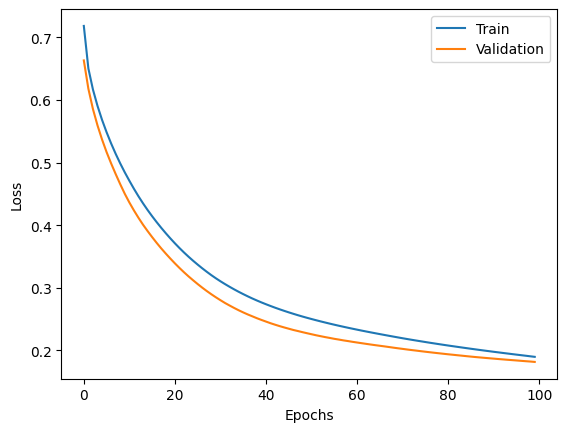
\includegraphics{LossEpochGraph.png}
    \caption{Loss/Epoch Grafiği}
    \label{fig:my_label}
\end{figure}

\newpage
\subsection{(10 Puan)} \textbf{SEED=öğrenci numaranız set ettikten sonra altıncı haftada ödev olarak verdiğim gibi earlystopping'deki en iyi modeli kullanarak, Prensesi İyileştir test setinden accuracy, F1, precision ve recall değerlerini hesaplayan kodu yazın ve sonucu da aşağı yapıştırın. \%80'den fazla başarı bekliyorum test setinden. Daha düşükse başarı oranınız, nerede hata yaptığınızı bulmaya çalışın. \%90'dan fazla başarı almak mümkün (ben denedim).}


\begin{python}
best_model_params = None
best_val_loss = float('inf')
patience = 20
counter = 0

for epoch in range(epochs):
    # Train
    model.train()
    train_loss = 0.0
    for i in range(0, len(train_data), batch_size):
        # Get batch of data
        batch_data = train_data[i:i+batch_size]
        batch_labels = train_labels[i:i+batch_size]
        # Zero the gradients
        optimizer.zero_grad()
        # Forward pass
        outputs = model(batch_data)
        loss = criterion(outputs, batch_labels.view(-1, 1))
        # Backward pass and optimization
        loss.backward()
        optimizer.step()
        train_loss += loss.item() * batch_data.size(0)
    train_loss = train_loss / len(train_data)
    train_losses.append(train_loss)
    
    # Validation
    model.eval()
    val_loss = 0.0
    with torch.no_grad():
        for i in range(0, len(val_data), batch_size):
            # Get batch of data
            batch_data = val_data[i:i+batch_size]
            batch_labels = val_labels[i:i+batch_size]            

            # Forward pass
            outputs = model(batch_data)
            loss = criterion(outputs, batch_labels.view(-1, 1))
            val_loss += loss.item() * batch_data.size(0)
        val_loss = val_loss / len(val_data)
        val_losses.append(val_loss)
        
        # Check if validation loss is the best so far
        if val_loss < best_val_loss:
            best_val_loss = val_loss
            best_model_params = model
            counter = 0
        else:
            counter += 1
            
        # Early stopping condition
        if counter >= patience:
            #print(f'Early stopping at epoch {epoch+1}')
            print("Validation loss hasn't improved for {} epochs. Stopping training early.".format(patience))
            break
    
    # Print epoch and loss
    if (epoch+1) % 10 == 0:
        print(f'Epoch [{epoch+1}/{epochs}], Train Loss: {train_loss:.4f}, Validation Loss: {val_loss:.4f}')

# Compute validation accuracy, precision, recall and F1 score
    tp = 0  # True positives
    fp = 0  # False positives
    tn = 0  # True negatives
    fn = 0  # False negatives
    best_model_params.eval()
    with torch.no_grad():
        for i in range(0, len(test_data), batch_size):
            # Get batch of data
            batch_data = test_data[i:i+batch_size]
            batch_labels = test_labels[i:i+batch_size]

            # Forward pass
            outputs = best_model_params(batch_data)
            predicted_labels = (outputs >= 0.5).float()

            # Update confusion matrix
            tp += torch.sum(predicted_labels * batch_labels).item()
            fp += torch.sum(predicted_labels * (1 - batch_labels)).item()
            tn += torch.sum((1 - predicted_labels) * (1 - batch_labels)).item()
            fn += torch.sum((1 - predicted_labels) * batch_labels).item()

            # Compute validation loss
            loss = criterion(outputs, batch_labels.view(-1, 1))
            val_loss += loss.item() * batch_data.size(0)
        val_loss = val_loss / len(test_data)

    # Compute accuracy, precision, recall and F1 score
    accuracy = (tp + tn) / (tp + tn + fp + fn)
    precision = tp / (tp + fp)
    recall = tp / (tp + fn)
    f1 = 2 * precision * recall / (precision + recall)

    print(f'Test Accuracy: {accuracy:.4f}, Test Precision: {precision:.4f}, Test Recall: {recall:.4f}, Test F1: {f1:.4f}')
\end{python}

Test Accuracy: 0.9339, Test Precision: 0.9517, Test Recall: 0.9149, Test F1: 0.9330


\subsection{(5 Puan)} \textbf{Tüm kodların CPU'da çalışması ne kadar sürüyor hesaplayın. Sonra to device yöntemini kullanarak modeli ve verileri GPU'ya atıp kodu bir de böyle çalıştırın ve ne kadar sürdüğünü hesaplayın. Süreleri aşağıdaki tabloya koyun. GPU için Google Colab ya da Kaggle'ı kullanabilirsiniz, iki ortam da her hafta saatlerce GPU hakkı veriyor.}

\begin{table}[ht!]
    \centering
    \caption{Tüm Kodların CPU ve GPU'da Çalışma Süresi}
    \begin{tabular}{c|c}
        Ortam & Süre (saniye) \\\hline
        CPU & 18 sn \\
        GPU & 14 sn\\
    \end{tabular}
    \label{tab:my_table}
\end{table}

\subsection{(3 Puan)} \textbf{Modelin eğitim setine overfit etmesi için elinizden geldiği kadar kodu gereken şekilde değiştirin, validasyon loss'unun açıkça yükselmeye başladığı, training ve validation loss'ları içeren figürü aşağı koyun ve overfit için yaptığınız değişiklikleri aşağı yazın. Overfit, tam bir çanak gibi olmalı ve yükselmeli. Ona göre parametrelerle oynayın.}

Learning Rate değerini 0.001'den 0.01 yaptığımda modelim overfit etmiş oldu. Sonuç aşağıdaki grafikte görülmektedir:


\begin{figure}[ht!]
    \centering
    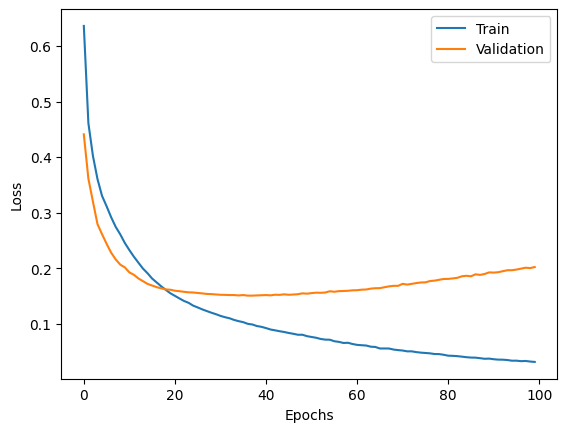
\includegraphics{overfitting lr = 0.01.png}
    \caption{Overfitting}
    \label{fig:my_picl}
\end{figure}
\newpage
\subsection{(2 Puan)} \textbf{Beşinci soruya ait tüm kodların ve cevapların olduğu jupyter notebook'un Github linkini aşağıdaki url'e koyun.}

\url{https://github.com/hesnacaliskan/Cure_the_Princess}

\section{(Toplam 10 Puan)} \textbf{Bir önceki sorudaki Prensesi İyileştir problemindeki yapay sinir ağınıza seçtiğiniz herhangi iki farklı regülarizasyon yöntemi ekleyin ve aşağıdaki soruları cevaplayın.} 

\subsection{(2 puan)} \textbf{Kodlarda regülarizasyon eklediğiniz kısımları aşağı koyun:} 

\begin{python}
class MLP(nn.Module):
    def __init__(self, input_size, hidden_size1, hidden_size2, output_size, reg_param):
        super(MLP, self).__init__()
        self.fc1 = nn.Linear(input_size, hidden_size1)
        self.relu1 = nn.ReLU()
        self.fc2 = nn.Linear(hidden_size1, hidden_size2)
        self.relu2 = nn.ReLU()
        self.fc3 = nn.Linear(hidden_size2, output_size)
        self.sigmoid = nn.Sigmoid()
        self.reg_param = reg_param
        
    def forward(self, x):
        out = self.fc1(x)
        out = self.relu1(out)
        out = self.fc2(out)
        out = self.relu2(out)
        out = self.fc3(out)
        out = self.sigmoid(out)
        return out
      
    def l2_regularization(self):
        l2_loss = 0.0
        for param in self.parameters():
            l2_loss += torch.norm(param)
        return l2_loss * self.reg_param
      
input_size = 13
hidden_size1 = 100
hidden_size2 = 50
output_size = 1
learning_rate = 0.001
epochs = 100
batch_size = 32
reg_param = 0.001 # L2 regularization parameter

model = MLP(input_size, hidden_size1, hidden_size2, output_size, reg_param)
criterion = nn.BCELoss()
optimizer = optim.SGD(model.parameters(), lr=learning_rate)

train_losses = []
val_losses = []
reg_losses = [] # L2 regularization losses

for epoch in range(epochs):
    # Train
    model.train()
    train_loss = 0.0
    for i in range(0, len(train_data), batch_size):
        # Get batch of data
        batch_data = train_data[i:i+batch_size]
        batch_labels = train_labels[i:i+batch_size]
        # Zero the gradients
        optimizer.zero_grad()
        # Forward pass
        outputs = model(batch_data)
        loss = criterion(outputs, batch_labels.view(-1, 1))
        # Add L2 regularization loss
        reg_loss = model.l2_regularization()
        loss += reg_loss
        # Backward pass and optimization
        loss.backward()
        optimizer.step()
        train_loss += loss.item() * batch_data.size(0)
    train_loss = train_loss / len(train_data)
    train_losses.append(train_loss)
    
    # Validation
    model.eval()
    val_loss = 0.0
    with torch.no_grad():
        for i in range(0, len(val_data), batch_size):
            # Get batch of data
            batch_data = val_data[i:i+batch_size]
            batch_labels = val_labels[i:i+batch_size]  
                    # Forward pass
            outputs = model(batch_data)
            loss = criterion(outputs, batch_labels.view(-1, 1))
            val_loss += loss.item() * batch_data.size(0)
        
            # L2 regularization
            l2_reg = torch.tensor(0.)
            for param in model.parameters():
              l2_reg += torch.norm(param, p=2)**2
        loss += 0.001 * l2_reg
        
        val_loss = val_loss / len(val_data)
        val_losses.append(val_loss)

  # Print epoch and loss
    if (epoch+1) % 10 == 0:
        print(f'Epoch [{epoch+1}/{epochs}], Train Loss: {train_loss:.4f}, Validation Loss: {val_loss:.4f}')
\end{python}

\subsection{(2 puan)} \textbf{Test setinden yeni accuracy, F1, precision ve recall değerlerini hesaplayıp aşağı koyun:}

Test Accuracy: 0.9197, Test Precision: 0.9158, Test Recall: 0.9253, Test F1: 0.9205


\subsection{(5 puan)} \textbf{Regülarizasyon yöntemi seçimlerinizin sebeplerini ve sonuçlara etkisini yorumlayın:}

Veri setinin sadece sayısal verilerden oluşması, çok sayıda özellik içermesi  ve bu özelliklerin etkisinin birbirinden bağımsız olmadığını düşünmemden dolayı L2 Regülarizasyonunu tercih ettim. Epoch/Loss grafiğine baktığımda tatmin edici bir sonuç elde ettim. Test setiyle modeli değerlendirdiğimde normalde Earlystopping olmadan elde ettiğim test accuracy değeri 0.9054 iken Regülarizasyon ile birlikte 0.9197 oldu. Modelin performansı açısından değerlendirmek istersem iyileştirmekten ziyade daha uzun süre çalıştığını kaydettim.


\subsection{(1 puan)} \textbf{Sonucun github linkini  aşağıya koyun:}

\url{https://github.com/hesnacaliskan/Cure_the_Princess_Regularization}

\end{document}